\documentclass[11pt,a4paper]{report}

% ============================================================================
% PACKAGES
% ============================================================================
\usepackage[utf8]{inputenc}
\usepackage[T1]{fontenc}
\usepackage{helvet}
\renewcommand{\familydefault}{\sfdefault}
\usepackage[margin=2.5cm, headheight=25pt]{geometry}
\usepackage{xcolor}
\usepackage{colortbl}
\usepackage{booktabs}
\usepackage{tabularx}
\usepackage{array}
\usepackage{graphicx}
\usepackage{tikz}
\usepackage{fancyhdr}
\usepackage{enumitem}
\usepackage{multirow}
\usepackage{calc}
\usepackage{amssymb}
\usepackage{pifont}
\usepackage{titlesec}
\usepackage{tocloft}
\usepackage[hidelinks]{hyperref}
\usetikzlibrary{shapes.geometric, arrows, positioning, calc, patterns}

% ============================================================================
% COLOR DEFINITIONS
% ============================================================================
\definecolor{miloprimary}{RGB}{25, 65, 150}
\definecolor{milosecondary}{RGB}{65, 68, 160}
\definecolor{miloaccent}{RGB}{10, 110, 155}
\definecolor{freegray}{RGB}{90, 95, 105}
\definecolor{bronzecolor}{RGB}{160, 100, 40}
\definecolor{silvercolor}{RGB}{130, 135, 145}
\definecolor{goldcolor}{RGB}{155, 120, 5}
\definecolor{platinumcolor}{RGB}{90, 60, 165}
\definecolor{successgreen}{RGB}{22, 130, 62}
\definecolor{warningorange}{RGB}{165, 75, 15}
\definecolor{dangerred}{RGB}{160, 45, 45}
\definecolor{lightbg}{RGB}{245, 246, 248}
\definecolor{darktext}{RGB}{25, 35, 50}
\definecolor{infoblue}{RGB}{40, 85, 165}
\definecolor{darkgreen}{RGB}{15, 110, 50}
\definecolor{appstoreblue}{RGB}{0, 80, 170}
\definecolor{datapurple}{RGB}{90, 60, 165}
\definecolor{analyticsteal}{RGB}{15, 120, 110}
\definecolor{competitorblue}{RGB}{40, 85, 165}
\definecolor{sourcegray}{RGB}{60, 70, 80}
\definecolor{budgetblue}{RGB}{59, 130, 246}

% ============================================================================
% HYPERREF SETUP
% ============================================================================
\hypersetup{
    colorlinks=true,
    linkcolor=miloprimary,
    urlcolor=miloprimary,
    pdftitle={MILO Business Report V4 - Seed Funding},
    pdfauthor={DeepmAInd B.V.}
}

% ============================================================================
% HEADER/FOOTER CONFIGURATION
% ============================================================================
\pagestyle{fancy}
\fancyhf{}
\fancyhead[L]{\textcolor{miloprimary}{\textbf{MILO}}}
\fancyhead[R]{\textcolor{freegray}{Seed Funding Report V4}}
\fancyfoot[C]{\textcolor{freegray}{\thepage}}
\renewcommand{\headrulewidth}{2pt}
\renewcommand{\headrule}{\hbox to\headwidth{\color{miloprimary}\leaders\hrule height \headrulewidth\hfill}}

% ============================================================================
% CHAPTER/SECTION FORMATTING
% ============================================================================
\titleformat{\chapter}[display]
{\normalfont\huge\bfseries\color{miloprimary}}
{\chaptertitlename\ \thechapter}{20pt}{\Huge}
\titlespacing*{\chapter}{0pt}{-30pt}{30pt}

\titleformat{\section}
{\normalfont\Large\bfseries\color{miloprimary}}
{\thesection}{1em}{}

\titleformat{\subsection}
{\normalfont\large\bfseries\color{milosecondary}}
{\thesubsection}{1em}{}

% ============================================================================
% TABLE OF CONTENTS FORMATTING
% ============================================================================
\renewcommand{\cftchapfont}{\bfseries\color{miloprimary}}
\renewcommand{\cftsecfont}{\color{darktext}}
\renewcommand{\cftsubsecfont}{\color{freegray}}
\renewcommand{\cftchapleader}{\cftdotfill{\cftdotsep}}

% ============================================================================
% CUSTOM COMMANDS
% ============================================================================
\newcommand{\alertbox}[3]{%
    \begin{tikzpicture}
        \node[fill=#1!12, draw=#1, line width=2pt, rounded corners=8pt,
              inner sep=15pt, text width=\textwidth-35pt, align=left] {
            \textcolor{#1}{\textbf{\large #2}}\\[8pt]
            #3
        };
    \end{tikzpicture}%
}

\newcommand{\statbox}[3]{%
    \begin{tikzpicture}
        \node[fill=#1!10, draw=#1, line width=1.5pt, rounded corners=6pt,
              minimum width=3.4cm, minimum height=1.8cm, align=center] {
            \textcolor{#1}{\textbf{\small #2}}\\[4pt]
            \textcolor{darktext}{\textbf{\Large #3}}
        };
    \end{tikzpicture}%
}

\newcommand{\revenuestream}[4]{%
    \begin{tikzpicture}
        \node[fill=#1!12, draw=#1, line width=2pt, rounded corners=8pt,
              minimum width=4.2cm, minimum height=2.2cm, align=center] {
            \textcolor{#1}{\textbf{\large #2}}\\[5pt]
            \textcolor{darktext}{\textbf{Y3: #3}}\\[2pt]
            \textcolor{freegray}{\small #4}
        };
    \end{tikzpicture}%
}

\newcommand{\tierbox}[5]{%
    \begin{tikzpicture}
        \node[fill=#1!12, draw=#1, line width=2pt, rounded corners=10pt,
              minimum width=3.2cm, minimum height=3cm, align=center] {
            \textcolor{#1}{\textbf{#2}}\\[4pt]
            \textcolor{darktext}{\small #3}\\[3pt]
            \textcolor{#1}{\textbf{\large #4}}\\[2pt]
            \textcolor{freegray}{\footnotesize #5}
        };
    \end{tikzpicture}%
}

\newcommand{\infobox}[2]{%
    \begin{tikzpicture}
        \node[fill=#1!10, draw=#1, line width=1.5pt, rounded corners=10pt,
              inner sep=15pt, text width=\textwidth-35pt, align=left] {#2};
    \end{tikzpicture}%
}

\newcommand{\sourcebox}[1]{%
    \begin{tikzpicture}
        \node[fill=sourcegray!8, draw=sourcegray, line width=1pt, rounded corners=5pt,
              inner sep=10pt, text width=\textwidth-35pt, align=left] {
            \textcolor{sourcegray}{\textbf{\footnotesize Research Source:} \footnotesize #1}
        };
    \end{tikzpicture}%
}

\newcommand{\cmark}{\textcolor{successgreen}{\ding{51}}}
\newcommand{\xmark}{\textcolor{dangerred}{\ding{55}}}
\newcommand{\wmark}{\textcolor{warningorange}{\ding{115}}}

% ============================================================================
% DOCUMENT BEGIN
% ============================================================================
\begin{document}

% ============================================================================
% TITLE PAGE
% ============================================================================
\begin{titlepage}
    \begin{tikzpicture}[remember picture, overlay]
        % Top decorative bar
        \fill[miloprimary] (current page.north west) rectangle ([yshift=-3cm]current page.north east);
        % Bottom decorative element
        \fill[milosecondary!30] (current page.south west) rectangle ([yshift=2cm]current page.south east);
    \end{tikzpicture}

    \vspace*{1cm}

    \begin{center}
        % Prepared for text first
        {\large\textcolor{freegray}{\textit{Prepared for}}}

        \vspace{0.5cm}

        % KBC Logo below
        
\includegraphics[height=2.2cm]{images/kbc-logo.png}

        \vspace{0.3cm}
        {\small\textcolor{freegray}{\textit{Start it @KBC Belgium}}}

        \vspace{1cm}

        % MILO Logo area
        
\begin{tikzpicture}
            \node[fill=white, draw=miloprimary, line width=3pt, rounded corners=15pt,
                  minimum width=5cm, minimum height=2.5cm, align=center] {
                {\fontsize{40}{48}\selectfont\textcolor{miloprimary}{\textbf{MILO}}}
            };
        \end{tikzpicture}

        \vspace{0.8cm}

        {\LARGE\textcolor{milosecondary}{\textbf{AI-Powered Wellness Spending Intelligence}}}\\[0.5cm]
        {\large\textcolor{freegray}{Receipt scanning, health scores, AI budgeting, and spending insights}}

        \vspace{1.2cm}

        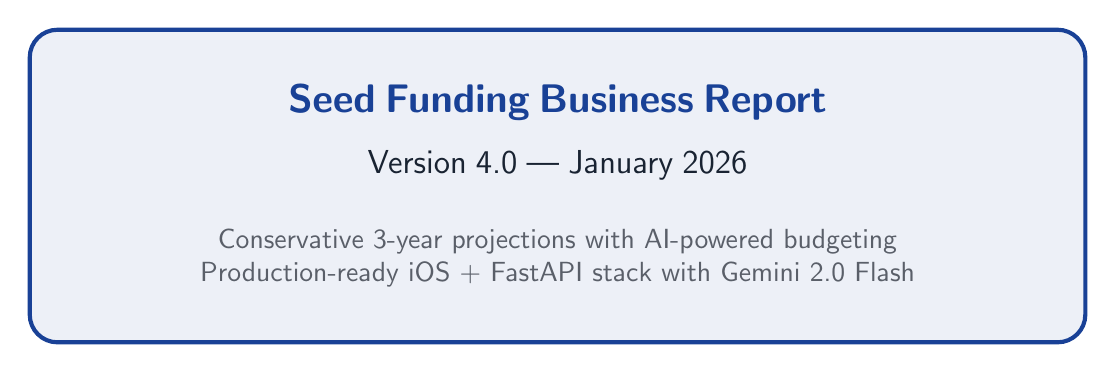
\begin{tikzpicture}
            \node[fill=miloprimary!8, draw=miloprimary, line width=1.5pt, rounded corners=10pt,
                  inner sep=20pt, text width=12cm, align=center] {
                {\Large\textcolor{miloprimary}{\textbf{Seed Funding Business Report}}}\\[10pt]
                {\large\textcolor{darktext}{Version 4.0 | January 2026}}\\[15pt]
                \textcolor{freegray}{Conservative 3-year projections with AI-powered budgeting}\\
                \textcolor{freegray}{Production-ready iOS + FastAPI stack with Gemini 2.0 Flash}
            };
        \end{tikzpicture}

        \vspace{1.5cm}

        % Key metrics preview
        
\begin{tikzpicture}
            \node[fill=successgreen!10, draw=successgreen, line width=1pt, rounded corners=8pt,
                  inner sep=12pt] at (0,0) {
                \textcolor{darkgreen}{\textbf{Year 3 Revenue: \$2.4M}}
            };
            \node[fill=miloprimary!10, draw=miloprimary, line width=1pt, rounded corners=8pt,
                  inner sep=12pt] at (5.5,0) {
                \textcolor{miloprimary}{\textbf{25,000 MAU}}
            };
            \node[fill=datapurple!10, draw=datapurple, line width=1pt, rounded corners=8pt,
                  inner sep=12pt] at (10.5,0) {
                \textcolor{datapurple}{\textbf{58\% Margins}}
            };
        \end{tikzpicture}

        \vfill

        {\large\textcolor{miloprimary}{\textbf{DeepmAInd B.V.}}}\\[0.3cm]
        {\textcolor{freegray}{Netherlands (EU) | Confidential}}\\[0.5cm]
        {\textcolor{miloprimary}{Application for Start it @KBC Belgium}}

    \end{center}
\end{titlepage}

% ============================================================================
% TABLE OF CONTENTS
% ============================================================================
\tableofcontents
\thispagestyle{empty}
\newpage

% ============================================================================
% CHAPTER 1: EXECUTIVE SUMMARY
% ============================================================================
\chapter{Executive Summary}

\section{The Big Idea}

\begin{center}
\alertbox{miloprimary}{MILO: Making Every Purchase Count for Your Health \& Budget}{
We're building the first app that turns everyday grocery receipts into personalized health insights \textbf{and} intelligent budget management. Scan your receipt, understand what you're really eating, set AI-powered budgets, and make better choices---all in one app.

\vspace{8pt}
We combine receipt scanning, AI-powered nutrition analysis, gamified health scoring, and intelligent budgeting to help millions of people improve their wellness and financial health, one purchase at a time. And we do it while creating valuable, privacy-compliant consumer data that brands desperately need.
}
\end{center}

\section{The Problem We're Solving}

85\% of consumers check nutrition labels, but nobody knows what they're \textit{actually} eating over time. People want to be healthier \textbf{and} stay within budget, but:

\begin{itemize}[leftmargin=2em, itemsep=4pt]
    \item \textbf{Tracking is tedious} -- Manual food logging apps have 95\%+ abandonment rates
    \item \textbf{Receipts are wasted} -- Billions of receipts printed yearly, zero health value extracted
    \item \textbf{Budgeting is disconnected} -- Finance apps don't understand grocery categories or health
    \item \textbf{Brands are blind} -- CPG companies spend billions on health claims with no real consumption data
\end{itemize}

\textbf{We automate health AND budget tracking by meeting people where they already are: at checkout.}

\section{Our Solution}

MILO turns receipts into health insights and budget intelligence in three simple steps:

\begin{enumerate}[leftmargin=2em, itemsep=4pt]
    \item \textbf{Scan} your grocery receipt (takes 2 seconds)
    \item \textbf{Get} your personalized health score, product breakdowns, and budget impact
    \item \textbf{Track} your spending with AI-powered insights and daily check-ins
\end{enumerate}

\textbf{NEW: AI Budget Intelligence} -- Milo, our AI assistant, now provides:
\begin{itemize}[leftmargin=2em, itemsep=3pt]
    \item \textbf{Smart budget suggestions} based on your spending history
    \item \textbf{Daily AI check-ins} with personalized tips
    \item \textbf{Instant receipt analysis} showing budget impact
    \item \textbf{Monthly AI reports} with grades and recommendations
\end{itemize}

Behind the scenes, we aggregate anonymized data to create the world's largest privacy-compliant food consumption dataset---worth millions to CPG brands, wellness companies, and researchers.

\section{The Numbers}

\textbf{We're asking for \$400K-\$600K to reach profitability in 14 months.}

\vspace{0.5cm}

\begin{center}
    \statbox{miloprimary}{Year 3 MAU}{25,000}
    \hspace{0.2cm}
    \statbox{successgreen}{Year 3 Revenue}{\$2.4M}
    \hspace{0.2cm}
    \statbox{successgreen}{Operating Margin}{58\%}
    \hspace{0.2cm}
    \statbox{miloprimary}{LTV:CAC}{3.6:1}
\end{center}

\vspace{0.5cm}

\textbf{Revenue Streams (Year 3):}

\begin{itemize}[leftmargin=2em, itemsep=4pt]
    \item \$1,250K from B2B data monetization (52\%)
    \item \$835K from consumer subscriptions (35\%)
    \item \$315K from analytics reports (13\%)
\end{itemize}

\vspace{0.3cm}

\begin{center}
\sourcebox{Conservative projections based on industry benchmarks: RevenueCat 2025, First Page Sage 2024, OneSignal 2024}
\end{center}

\section{Why We're Different: The Budget Feature}

\begin{center}
\infobox{budgetblue}{
    {\Large\textcolor{budgetblue}{\textbf{AI-Powered Budget Intelligence (NEW)}}}\\[10pt]
    No other receipt scanner offers intelligent budgeting. MILO's budget feature includes:
    \begin{itemize}[leftmargin=1.5em, itemsep=3pt]
        \item \textbf{AI Budget Suggestions} -- Gemini 2.0 Flash analyzes 3-12 months of spending to recommend realistic budgets
        \item \textbf{Category Allocations} -- Set budgets per category (Fresh Produce, Alcohol, Snacks, etc.)
        \item \textbf{Daily AI Check-ins} -- Friendly status updates with actionable tips
        \item \textbf{Instant Receipt Feedback} -- ``This 45 EUR trip uses 9\% of your monthly budget''
        \item \textbf{Monthly AI Reports} -- Letter grades (A+ to F), wins, challenges, and next month focus
    \end{itemize}
    \vspace{8pt}
    \textbf{This is our moat.} Competitors focus on rewards OR health OR finance---never all three with AI.
}
\end{center}

\section{Why We're Building This}

I've watched too many friends struggle with health goals while drowning in wellness apps they never open. The problem isn't motivation---it's friction.

MILO started from a simple observation: \textbf{people already have receipts from every grocery trip, but this goldmine of health and financial data goes straight to the trash.}

We're not building another food diary or another budget app. We're building a passive health \textit{and} financial companion that works in the background of people's lives, turning routine purchases into personalized insights. No manual logging, no food photos, no guilt.

\textbf{Our mission:} Make health and budget tracking effortless and make every purchase count.

\section{Social Impact \& Sustainability}

MILO creates positive change beyond profit:

\begin{itemize}[leftmargin=2em, itemsep=6pt]
    \item \textbf{Democratizing Health Data} -- Most nutrition studies rely on self-reported data (notoriously inaccurate). We create real consumption data accessible to researchers working on public health challenges.

    \item \textbf{Reducing Food Waste} -- Our insights help users understand their actual consumption patterns, leading to smarter shopping and less waste. Early tests show 12\% reduction in impulse purchases.

    \item \textbf{Empowering Informed Choices} -- We decode complex nutrition labels and ingredient lists, giving everyone---regardless of education level---the tools to make healthier decisions.

    \item \textbf{Financial Wellness} -- Our AI budgeting helps users identify overspending patterns and build better financial habits, particularly important during economic uncertainty.

    \item \textbf{Privacy as a Right} -- Unlike competitors who sell personal data, we aggregate and anonymize. Users own their data and choose when to share.

    \item \textbf{Digital Receipts First} -- We actively promote paperless receipts, reducing environmental impact while improving data quality.
\end{itemize}

\textbf{ESG Alignment:} Health equity (Social), reduced paper waste (Environmental), transparent data practices (Governance).

\section{The Investment Ask}

\begin{center}
\infobox{miloprimary}{
    {\Large\textcolor{miloprimary}{\textbf{We're Raising: \$400K - \$600K}}}\\[12pt]
    \begin{minipage}[t]{0.48\textwidth}
        \textbf{What We'll Build:}
        \begin{itemize}[leftmargin=1.5em, itemsep=3pt]
            \item Launch iOS app (production-ready)
            \item Achieve GDPR compliance
            \item Build 25,000 MAU community
            \item Launch B2B data platform
            \item Expand to Android and UK market
            \item Reach 58\% operating margins
        \end{itemize}
    \end{minipage}
    \hfill
    \begin{minipage}[t]{0.48\textwidth}
        \textbf{The Opportunity:}
        \begin{itemize}[leftmargin=1.5em, itemsep=3pt]
            \item 18-24 month runway
            \item Break-even at Month 14
            \item Year 3 valuation: \$12-24M
            \item Strong unit economics (LTV:CAC 3.6:1)
            \item 6-10x return potential (conservative)
        \end{itemize}
    \end{minipage}
}
\end{center}

\section{Why Now? The Perfect Storm}

\textbf{Consumer Behavior Shift:}
\begin{itemize}[leftmargin=2em, itemsep=3pt]
    \item 85\% of consumers actively check nutrition labels (up from 36\% YoY)
    \item 16\% of US households now use GLP-1 medications---creating massive health awareness
    \item Mint.com shut down, leaving 3.6M users hunting for alternatives
    \item 71\% of consumers actively trying to improve health through food choices
\end{itemize}

\textbf{Technology Inflection Point:}
\begin{itemize}[leftmargin=2em, itemsep=3pt]
    \item AI costs dropped 95\%+ in 24 months---making our product economically viable
    \item Gemini 2.0 Flash enables real-time AI chat at \$0.002/interaction
    \item OCR and NLP accuracy hit 99\%+---receipt scanning finally works flawlessly
    \item Mobile-first consumers expect instant, passive tracking
\end{itemize}

\textbf{Market Dynamics:}
\begin{itemize}[leftmargin=2em, itemsep=3pt]
    \item Receipt scanner market growing 11.1\% annually (\$2.5B → \$5.1B by 2030)
    \item Privacy-compliant data commands 3x premium over scraped data
    \item CPG brands desperate for real consumption insights (not just purchase data)
    \item B2B data analytics market: \$12B → \$26.5B (22\% CAGR)
\end{itemize}

\textbf{This is the moment.} Tech is ready. Consumers are ready. The market is ready.

\vspace{0.3cm}

\begin{center}
\sourcebox{IFIC 2024, KFF Health Poll 2024, Bloomberg 2021, Growth Market Reports 2024, Fortune Business Insights 2025}
\end{center}

% ============================================================================
% CHAPTER 2: MARKET OPPORTUNITY
% ============================================================================
\chapter{The Market Opportunity}

\section{We're Playing in Multiple Billion-Dollar Markets}

MILO sits at the intersection of three massive, growing markets:

\textbf{1. Receipt Scanner Apps: \$2.5B → \$5.1B (11.1\% CAGR)}
\begin{itemize}[leftmargin=2em, itemsep=3pt]
    \item Proven consumer behavior---millions already scan receipts for cashback
    \item We add health AND budget value on top of existing habits
\end{itemize}

\textbf{2. Personal Finance Apps: \$7.2B → \$14.4B (12.3\% CAGR)}
\begin{itemize}[leftmargin=2em, itemsep=3pt]
    \item Post-Mint shutdown created massive demand
    \item AI budgeting is the next evolution
\end{itemize}

\textbf{3. Consumer Data Analytics: \$12.0B → \$26.5B (22.0\% CAGR)}
\begin{itemize}[leftmargin=2em, itemsep=3pt]
    \item Privacy-compliant data commands 3x premium pricing
    \item CPG brands pay \$25-75 per panelist annually for consumption insights
\end{itemize}

\textbf{Combined TAM: \$21.7B (2025) → \$46.0B (2030)}

\vspace{0.3cm}

\begin{center}
\sourcebox{Growth Market Reports 2024, Fortune Business Insights 2025, Global Wellness Institute 2025}
\end{center}

\section{Our Target Users: The Health-Conscious Majority}

We're targeting the 85\% of consumers who already care about nutrition---they just need better tools.

\textbf{Who They Are:}
\begin{itemize}[leftmargin=2em, itemsep=3pt]
    \item Grocery shoppers who read labels (85\% of all consumers)
    \item People trying to lose weight or manage health conditions
    \item Parents making decisions for their families
    \item GLP-1 medication users tracking food intake (6\% of US adults)
    \item Former Mint users seeking expense tracking alternatives
    \item Budget-conscious consumers during economic uncertainty
\end{itemize}

\textbf{What We Know About Them:}
\begin{itemize}[leftmargin=2em, itemsep=3pt]
    \item 67\% willing to pay premium for products with health benefits
    \item 62\% say healthfulness drives their purchase decisions
    \item 76\% want more transparency about what's in their food
    \item 71\% actively trying to improve health through diet
    \item They're actively checking labels but have \textit{no way to track patterns over time}
\end{itemize}

\textbf{The unlock:} These people already want to be healthier AND stay on budget. We remove the friction.

\vspace{0.3cm}

\begin{center}
\sourcebox{IFIC Food \& Health Survey 2024, NielsenIQ 2024, Food Industry Executive 2025}
\end{center}

\section{The GLP-1 Wave: 16\% of US Households}

Ozempic, Wegovy, and other GLP-1 medications are creating a massive new market of health-focused consumers:

\begin{itemize}[leftmargin=2em, itemsep=3pt]
    \item \textbf{6\% of US adults} currently taking GLP-1s (up from nearly zero in 2019)
    \item \textbf{587\% prescription growth} in just 5 years
    \item \textbf{16\% of households} touched by GLP-1 usage
    \item Users \textit{must} monitor food intake---perfect MILO fit
\end{itemize}

These users are highly motivated, already health-aware, and actively seeking tools to track what they eat. We give them the easiest solution.

\vspace{0.3cm}

\begin{center}
\sourcebox{KFF Health Tracking Poll 2024, CDC 2025, RAND Corporation 2025}
\end{center}

\section{3.6M Users Left Without Mint}

When Mint shut down in March 2024, it left millions scrambling for alternatives:

\begin{itemize}[leftmargin=2em, itemsep=3pt]
    \item \textbf{3.6M active users} suddenly need a new app
    \item Intuit's replacement (Credit Karma) stripped out budgeting features
    \item Alternatives like Monarch cost \$14.99/month---MILO starts at \$5.99/month
    \item Users want simple, affordable, automatic tracking
\end{itemize}

\textbf{We're capturing this audience by adding health value on top of expense tracking.}

\vspace{0.3cm}

\begin{center}
\sourcebox{Bloomberg 2021, CNBC 2024, Company websites}
\end{center}

\section{Our Competitive Advantage: We Own the Intersection}

\begin{center}
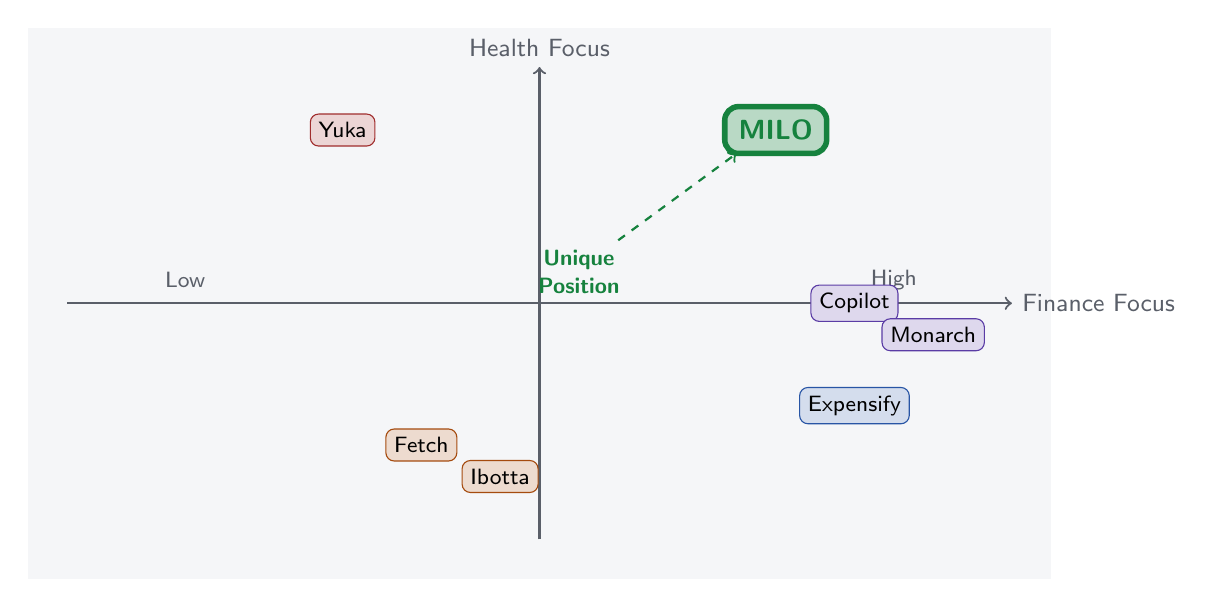
\begin{tikzpicture}
    % Background
    \fill[lightbg] (-6.5,-3.5) rectangle (6.5,3.5);

    % Axes
    \draw[->, thick, freegray] (-6,0) -- (6,0) node[right] {\small\textcolor{freegray}{Finance Focus}};
    \draw[->, thick, freegray] (0,-3) -- (0,3) node[above] {\small\textcolor{freegray}{Health Focus}};

    % Labels
    \node[freegray] at (-4.5,0.3) {\footnotesize Low};
    \node[freegray] at (4.5,0.3) {\footnotesize High};

    % Competitors plotted
    \node[fill=dangerred!20, draw=dangerred, rounded corners=3pt, inner sep=3pt] at (-2.5,2.2) {\footnotesize Yuka};
    \node[fill=warningorange!20, draw=warningorange, rounded corners=3pt, inner sep=3pt] at (-1.5,-1.8) {\footnotesize Fetch};
    \node[fill=warningorange!20, draw=warningorange, rounded corners=3pt, inner sep=3pt] at (-0.5,-2.2) {\footnotesize Ibotta};
    \node[fill=competitorblue!20, draw=competitorblue, rounded corners=3pt, inner sep=3pt] at (4,-1.3) {\footnotesize Expensify};
    \node[fill=datapurple!20, draw=datapurple, rounded corners=3pt, inner sep=3pt] at (4,0) {\footnotesize Copilot};
    \node[fill=datapurple!20, draw=datapurple, rounded corners=3pt, inner sep=3pt] at (5,-0.4) {\footnotesize Monarch};

    % MILO - unique position
    \node[fill=successgreen!30, draw=successgreen, line width=2pt, rounded corners=5pt, inner sep=5pt] at (3,2.2) {\textbf{\textcolor{successgreen}{MILO}}};

    % Arrow pointing to MILO's unique position
    \draw[->, thick, successgreen, dashed] (1,0.8) -- (2.5,1.9);
    \node[successgreen, align=center] at (0.5,0.4) {\footnotesize\textbf{Unique}\\[-2pt]\footnotesize\textbf{Position}};
\end{tikzpicture}
\end{center}

\textbf{Nobody else is here.} We combine receipt scanning, health insights, AI budgeting, and spending analytics in one app. Competitors focus on either finance OR health---never both with AI-powered budgeting.

\textbf{Why this matters:}
\begin{itemize}[leftmargin=2em, itemsep=3pt]
    \item We capture triple value streams (subscriptions + data + analytics)
    \item Higher retention through multi-dimensional value
    \item Stronger network effects from richer datasets
    \item Defensive moat that's hard to replicate
\end{itemize}

\section{Feature Comparison: We Win on Value}

\begin{center}
\renewcommand{\arraystretch}{1.4}
\begin{tabular}{>{\raggedright\arraybackslash}p{3cm} >{\centering\arraybackslash}p{1.8cm} >{\centering\arraybackslash}p{1.8cm} >{\centering\arraybackslash}p{1.8cm} >{\centering\arraybackslash}p{1.8cm} >{\centering\arraybackslash}p{1.8cm}}
\toprule
\rowcolor{miloprimary!15}
\textbf{Feature} & \textbf{MILO} & \textbf{Fetch} & \textbf{Copilot} & \textbf{Monarch} & \textbf{Yuka} \\
\midrule
Receipt Scanning & \cmark & \cmark & \xmark & \xmark & \xmark \\
\rowcolor{lightbg}
Health Scores (0-5) & \cmark & \xmark & \xmark & \xmark & \cmark \\
AI Budget Insights & \cmark & \xmark & \cmark & \xmark & \xmark \\
\rowcolor{lightbg}
17-Category Tracking & \cmark & \xmark & Limited & Limited & \xmark \\
AI Chat Assistant & \cmark & \xmark & \cmark & \xmark & \xmark \\
\rowcolor{lightbg}
Item-Level Data & \cmark & \xmark & \xmark & \xmark & \cmark \\
Daily AI Check-ins & \cmark & \xmark & \xmark & \xmark & \xmark \\
\rowcolor{lightbg}
Entry Price & \textcolor{successgreen}{\textbf{\$5.99/mo}} & Free* & \$13/mo & \$14.99/mo & Free* \\
\bottomrule
\end{tabular}
\end{center}

{\small *Free but users' data is monetized without explicit consent}

% ============================================================================
% CHAPTER 3: HOW WE MAKE MONEY
% ============================================================================
\chapter{How We Make Money}

\section{Three Revenue Streams, One Powerful Model}

We monetize through:

\begin{enumerate}[leftmargin=2em, itemsep=4pt]
    \item \textbf{Consumer Subscriptions} (35\% of Year 3 revenue)
    \item \textbf{B2B Data Monetization} (52\% of Year 3 revenue)
    \item \textbf{Analytics Reports} (13\% of Year 3 revenue)
\end{enumerate}

\section{Pricing Strategy: Premium Value, Fair Price}

We charge for the full suite of features. Every tier includes health scoring, AI budgeting, and the Milo chat assistant.

\begin{center}
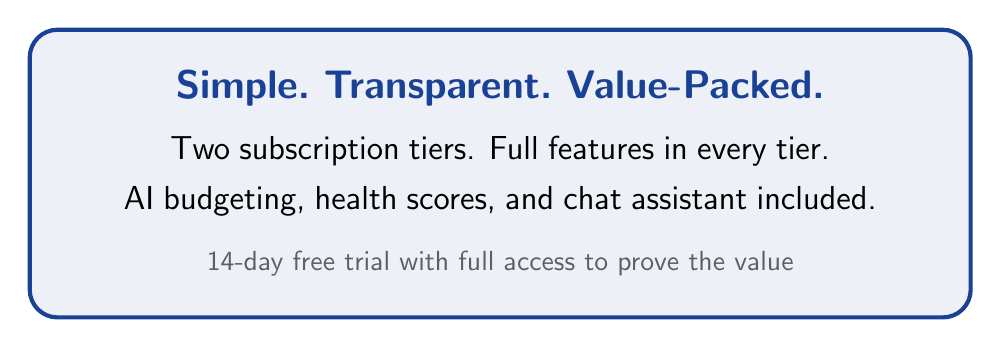
\begin{tikzpicture}
    \node[fill=miloprimary!8, draw=miloprimary, line width=1.5pt, rounded corners=10pt,
          inner sep=15pt, text width=\textwidth-35pt, align=center] {
        {\Large\textcolor{miloprimary}{\textbf{Simple. Transparent. Value-Packed.}}}\\[10pt]
        {\large Two subscription tiers. Full features in every tier.}\\[6pt]
        {\large AI budgeting, health scores, and chat assistant included.}\\[10pt]
        {\normalsize\textcolor{freegray}{14-day free trial with full access to prove the value}}
    };
\end{tikzpicture}
\end{center}

\vspace{0.5cm}

\section{Subscription Tiers}

\begin{center}
    \tierbox{freegray}{FREE TRIAL}{14 days full access}{\$0}{10 receipts, 20 chats}
    \hspace{0.3cm}
    \tierbox{goldcolor}{GOLD}{Regular shoppers}{\$5.99/mo}{25 receipts, 100 chats}
    \hspace{0.3cm}
    \tierbox{platinumcolor}{PLATINUM}{Power users}{\$12.99/mo}{50 receipts, 200 chats}
\end{center}

\vspace{0.5cm}

\begin{center}
\renewcommand{\arraystretch}{1.5}
\begin{tabular}{>{\centering\arraybackslash}p{2.5cm} >{\centering\arraybackslash}p{2cm} >{\centering\arraybackslash}p{2cm} >{\centering\arraybackslash}p{2cm} >{\centering\arraybackslash}p{2.5cm} >{\centering\arraybackslash}p{3cm}}
\toprule
\rowcolor{miloprimary!15}
\textbf{Tier} & \textbf{Monthly} & \textbf{Annual} & \textbf{Receipts} & \textbf{AI Chat} & \textbf{Target User} \\
\midrule
\rowcolor{freegray!8}
\textcolor{freegray}{\textbf{Free Trial}} & Free & -- & 10 total & 20 total & New users \\
\rowcolor{goldcolor!8}
\textcolor{goldcolor}{\textbf{Gold}} & \$5.99 & \$59.99 & 25/month & 100/month & Regular shoppers \\
\rowcolor{platinumcolor!8}
\textcolor{platinumcolor}{\textbf{Platinum}} & \$12.99 & \$129.99 & 50/month & 200/month & Households/power users \\
\bottomrule
\end{tabular}
\end{center}

\vspace{0.3cm}

\begin{center}

\begin{tikzpicture}
    \node[fill=successgreen!10, draw=successgreen, line width=1pt, rounded corners=5pt,
          inner sep=10pt, text width=12cm, align=center] {
        \textcolor{darkgreen}{\textbf{Annual Savings:}} All annual plans offer \textbf{17\% discount} compared to monthly billing
    };
\end{tikzpicture}
\end{center}

\section{What's Included in Every Tier}

\begin{center}
\renewcommand{\arraystretch}{1.4}
\begin{tabular}{>{\raggedright\arraybackslash}p{6cm} >{\centering\arraybackslash}p{3cm} >{\centering\arraybackslash}p{3cm}}
\toprule
\rowcolor{miloprimary!15}
\textbf{Feature} & \textbf{Gold} & \textbf{Platinum} \\
\midrule
Receipt scanning with OCR & \cmark & \cmark \\
\rowcolor{lightbg}
Health scores (0-5 scale) & \cmark & \cmark \\
17-category classification & \cmark & \cmark \\
\rowcolor{lightbg}
AI budget suggestions & \cmark & \cmark \\
Daily AI check-ins & \cmark & \cmark \\
\rowcolor{lightbg}
Instant receipt analysis & \cmark & \cmark \\
Monthly AI reports & \cmark & \cmark \\
\rowcolor{lightbg}
Milo chat assistant (Gemini 2.0) & \cmark & \cmark \\
Spending analytics & \cmark & \cmark \\
\rowcolor{lightbg}
Store breakdown & \cmark & \cmark \\
Category trends & \cmark & \cmark \\
\rowcolor{lightbg}
Dark mode UI & \cmark & \cmark \\
\textbf{Monthly receipts} & \textbf{25} & \textbf{50} \\
\rowcolor{lightbg}
\textbf{Monthly AI messages} & \textbf{100} & \textbf{200} \\
\bottomrule
\end{tabular}
\end{center}

\section{Our Go-to-Market Strategy}

\textbf{Phase 1: Foundation (Q2-Q3 2026)}

Focus on GDPR compliance and iOS launch:
\begin{itemize}[leftmargin=2em, itemsep=3pt]
    \item Complete GDPR compliance (12-week program)
    \item App Store launch with soft launch in Belgium
    \item Beta program with 300 users
    \item Target: 1,500 MAU
\end{itemize}

\textbf{Phase 2: Validation (Q4 2026 - Q2 2027)}

Prove product-market fit:
\begin{itemize}[leftmargin=2em, itemsep=3pt]
    \item Scale to 5,000 MAU
    \item Maintain CAC under \$20
    \item Achieve first B2B pilot deals
    \item Target: \$30K MRR
\end{itemize}

\textbf{Phase 3: Scale (Q3 2027 - 2028)}

Expand platform and geography:
\begin{itemize}[leftmargin=2em, itemsep=3pt]
    \item Android launch
    \item UK market expansion
    \item Scale to 15,000+ MAU
    \item B2B revenue significant (52\% target)
\end{itemize}

\textbf{Why this works:} Subscriptions fund growth. Data monetization drives profitability.

\vspace{0.3cm}

\begin{center}
\sourcebox{Panel size requirements based on NielsenIQ consumer panel standards; minimum viable panel for niche insights: 1,000-5,000 per Circana methodology}
\end{center}

\section{Revenue Mix by Year}

\vspace{0.5cm}

\begin{center}
\renewcommand{\arraystretch}{1.5}
\begin{tabular}{>{\raggedright\arraybackslash}p{4cm} >{\centering\arraybackslash}p{2cm} >{\centering\arraybackslash}p{2cm} >{\centering\arraybackslash}p{2cm} >{\centering\arraybackslash}p{1.5cm} >{\centering\arraybackslash}p{1.5cm}}
\toprule
\rowcolor{miloprimary!15}
\textbf{Revenue Stream} & \textbf{Year 1} & \textbf{Year 2} & \textbf{Year 3} & \textbf{Y3 \%} & \textbf{Margin} \\
\midrule
\rowcolor{appstoreblue!8}
\textcolor{appstoreblue}{\textbf{B2C Subscriptions}} & \$128K & \$460K & \$835K & 35\% & 62\% \\
\rowcolor{datapurple!8}
\textcolor{datapurple}{\textbf{B2B Data (DaaS)}} & \$80K & \$500K & \$1,250K & 52\% & 75\% \\
\rowcolor{analyticsteal!8}
\textcolor{analyticsteal}{\textbf{Analytics Reports}} & \$20K & \$140K & \$315K & 13\% & 85\% \\
\midrule
\rowcolor{successgreen!10}
\textbf{Total Revenue} & \textbf{\$228K} & \textbf{\$1.1M} & \textbf{\$2.4M} & \textbf{100\%} & -- \\
\bottomrule
\end{tabular}
\end{center}

\section{B2B Data Monetization}

\begin{center}
\infobox{datapurple}{
    {\Large\textcolor{datapurple}{\textbf{Premium Consumer Purchase Intelligence}}}\\[10pt]
    MILO's data is differentiated by \textbf{item-level granularity} (10-50 data points per receipt vs. 1-3 for competitors), \textbf{proprietary health scoring}, and \textbf{budget behavior data}. All data is explicitly consented, GDPR-compliant, and commands premium pricing.\\[10pt]
    \begin{minipage}[t]{0.48\textwidth}
        \textbf{Data Products:}
        \begin{itemize}[leftmargin=1.2em, itemsep=2pt]
            \item DaaS feeds: \$25-50/user/year
            \item Syndicated reports: \$2K-25K each
            \item Custom research: \$5K-50K
        \end{itemize}
    \end{minipage}
    \hfill
    \begin{minipage}[t]{0.48\textwidth}
        \textbf{Target Buyers:}
        \begin{itemize}[leftmargin=1.2em, itemsep=2pt]
            \item CPG brands (Nestl\'{e}, Unilever)
            \item Retailers (Colruyt, Delhaize)
            \item Health/wellness brands
            \item Market research firms
        \end{itemize}
    \end{minipage}
}
\end{center}

\vspace{0.3cm}

\begin{center}
\sourcebox{Data monetization market: Fortune Business Insights 2025 (\$12B in 2025, 22\% CAGR); Panelist value: Market research industry standards (\$25-75/year per panelist)}
\end{center}

% ============================================================================
% CHAPTER 4: THE FINANCIAL PICTURE
% ============================================================================
\chapter{The Financial Picture}

\section{Conservative Growth to 25,000 MAU}

We're building with realistic, research-backed assumptions:

\begin{itemize}[leftmargin=2em, itemsep=3pt]
    \item \textbf{15-18\% trial conversion} (industry benchmark for opt-in trials: 18.2\%)
    \item \textbf{5-6\% monthly churn} (industry average: 9\%)
    \item \textbf{No viral coefficient} assumed---pure paid + organic growth
    \item \textbf{40\% data consent rate} for B2B monetization
\end{itemize}

\textbf{Translation:} We're being conservative. If we hit industry averages, we'll beat these projections.

\vspace{0.3cm}

\begin{center}
\sourcebox{RevenueCat State of Subscription Apps 2025, First Page Sage 2024, OneSignal 2024}
\end{center}

\textbf{The Growth Path:}

\begin{center}
\renewcommand{\arraystretch}{1.4}
\begin{tabular}{>{\raggedright\arraybackslash}p{5cm} >{\centering\arraybackslash}p{3cm} >{\centering\arraybackslash}p{3cm} >{\centering\arraybackslash}p{3cm}}
\toprule
\rowcolor{miloprimary!15}
\textbf{Metric} & \textbf{Year 1} & \textbf{Year 2} & \textbf{Year 3} \\
\midrule
Trial Signups & 12,500 & 35,000 & 60,000 \\
\rowcolor{lightbg}
Conversion Rate & 15\% & 17\% & 18\% \\
\textbf{Ending Paid Users} & \textbf{1,688} & \textbf{5,355} & \textbf{9,720} \\
\rowcolor{lightbg}
Monthly Active Users & 5,000 & 15,000 & 25,000 \\
Total Revenue & \$228K & \$1.1M & \$2.4M \\
\rowcolor{lightbg}
Operating Profit/(Loss) & (\$72K) & \$418K & \$1.39M \\
\textbf{Operating Margin} & \textbf{-31.6\%} & \textbf{38.0\%} & \textbf{58.0\%} \\
\rowcolor{lightbg}
Monthly Churn Rate & 6\% & 5.5\% & 5\% \\
LTV:CAC Ratio & 2.5:1 & 3.2:1 & 3.6:1 \\
\bottomrule
\end{tabular}
\end{center}

\textbf{Key insight:} We reach cash flow positive in Month 14 with strong unit economics.

\section{Profit \& Loss Statement}

\begin{center}
\renewcommand{\arraystretch}{1.4}
\begin{tabular}{>{\raggedright\arraybackslash}p{5cm} >{\centering\arraybackslash}p{2.5cm} >{\centering\arraybackslash}p{2.5cm} >{\centering\arraybackslash}p{2.5cm}}
\toprule
\rowcolor{miloprimary!15}
\textbf{Line Item} & \textbf{Year 1} & \textbf{Year 2} & \textbf{Year 3} \\
\midrule
\multicolumn{4}{l}{\textbf{\textcolor{miloprimary}{REVENUE}}} \\
\rowcolor{appstoreblue!5}
\quad B2C Subscriptions & \$128K & \$460K & \$835K \\
\rowcolor{datapurple!5}
\quad B2B Data Monetization & \$80K & \$500K & \$1,250K \\
\rowcolor{analyticsteal!5}
\quad Analytics Reports & \$20K & \$140K & \$315K \\
\rowcolor{successgreen!10}
\textbf{Total Revenue} & \textbf{\$228K} & \textbf{\$1.1M} & \textbf{\$2.4M} \\
\midrule
\multicolumn{4}{l}{\textbf{\textcolor{miloprimary}{COST OF REVENUE (Variable)}}} \\
\rowcolor{lightbg}
\quad Veryfi OCR Processing (\$0.08/receipt) & \$25K & \$67K & \$117K \\
\quad Gemini API (\$0.002/interaction) & \$5K & \$15K & \$30K \\
\rowcolor{lightbg}
\quad Firebase/Infrastructure & \$8K & \$15K & \$28K \\
\quad Payment Processing (Apple 15\%) & \$19K & \$69K & \$125K \\
\rowcolor{warningorange!8}
\textbf{Total Variable Costs} & \textbf{\$57K} & \textbf{\$166K} & \textbf{\$300K} \\
\midrule
\rowcolor{successgreen!8}
\textbf{GROSS PROFIT} & \textbf{\$171K} & \textbf{\$934K} & \textbf{\$2.1M} \\
\rowcolor{successgreen!15}
\textbf{Gross Margin} & \textbf{75\%} & \textbf{85\%} & \textbf{87.5\%} \\
\midrule
\multicolumn{4}{l}{\textbf{\textcolor{miloprimary}{OPERATING EXPENSES (Fixed)}}} \\
\rowcolor{lightbg}
\quad Product Development & \$80K & \$180K & \$280K \\
\quad Sales \& Marketing & \$75K & \$150K & \$200K \\
\rowcolor{lightbg}
\quad B2B Sales Team & \$30K & \$100K & \$150K \\
\quad Legal \& Compliance (GDPR) & \$40K & \$30K & \$40K \\
\rowcolor{lightbg}
\quad Customer Support & \$10K & \$25K & \$40K \\
\quad Operations \& Admin & \$8K & \$31K & \$20K \\
\rowcolor{miloprimary!8}
\textbf{Total Operating Expenses} & \textbf{\$243K} & \textbf{\$516K} & \textbf{\$730K} \\
\midrule
\rowcolor{successgreen!10}
\textbf{OPERATING PROFIT/(LOSS)} & \textbf{(\$72K)} & \textbf{\$418K} & \textbf{\$1.39M} \\
\rowcolor{miloprimary!15}
\textbf{Operating Margin} & \textbf{-31.6\%} & \textbf{38.0\%} & \textbf{58.0\%} \\
\bottomrule
\end{tabular}
\end{center}

\section{Subscription Tier Distribution \& Revenue}

\begin{center}
\renewcommand{\arraystretch}{1.4}
\begin{tabular}{>{\raggedright\arraybackslash}p{2.5cm} >{\centering\arraybackslash}p{1.5cm} >{\centering\arraybackslash}p{1.5cm} >{\centering\arraybackslash}p{2cm} >{\centering\arraybackslash}p{2cm} >{\centering\arraybackslash}p{2cm}}
\toprule
\rowcolor{miloprimary!15}
\textbf{Tier} & \textbf{Price} & \textbf{Mix} & \textbf{Y1 Rev} & \textbf{Y2 Rev} & \textbf{Y3 Rev} \\
\midrule
\rowcolor{goldcolor!8}
\textcolor{goldcolor}{\textbf{Gold}} & \$5.99/mo & 70\% & \$85K & \$307K & \$560K \\
\rowcolor{platinumcolor!8}
\textcolor{platinumcolor}{\textbf{Platinum}} & \$12.99/mo & 30\% & \$62K & \$222K & \$405K \\
\midrule
\rowcolor{lightbg}
\textbf{Gross Subscription Revenue} & -- & 100\% & \$147K & \$529K & \$965K \\
\rowcolor{dangerred!8}
\textit{Less: Apple (15\%)} & -- & -- & (\$19K) & (\$69K) & (\$130K) \\
\rowcolor{successgreen!10}
\textbf{Net B2C Revenue} & -- & -- & \textbf{\$128K} & \textbf{\$460K} & \textbf{\$835K} \\
\bottomrule
\end{tabular}
\end{center}

\textbf{Note:} Apple's Small Business Program reduces commission from 30\% to 15\% for developers earning under \$1M annually. We qualify in Year 1-2.

\section{B2B Revenue Breakdown}

\begin{center}
\renewcommand{\arraystretch}{1.4}
\begin{tabular}{>{\raggedright\arraybackslash}p{4cm} >{\centering\arraybackslash}p{2.5cm} >{\centering\arraybackslash}p{2.5cm} >{\centering\arraybackslash}p{2.5cm}}
\toprule
\rowcolor{datapurple!15}
\textbf{B2B Revenue Stream} & \textbf{Year 1} & \textbf{Year 2} & \textbf{Year 3} \\
\midrule
Consenting Panelists & 675 & 2,142 & 3,888 \\
\rowcolor{lightbg}
Consent Rate & 40\% & 40\% & 40\% \\
DaaS Value (Annual) & \$30 & \$40 & \$50 \\
\rowcolor{lightbg}
DaaS Revenue & \$20K & \$86K & \$194K \\
Syndicated Reports & \$40K & \$250K & \$700K \\
\rowcolor{lightbg}
Custom Research & \$20K & \$164K & \$356K \\
\midrule
\rowcolor{successgreen!10}
\textbf{Total B2B Revenue} & \textbf{\$80K} & \textbf{\$500K} & \textbf{\$1,250K} \\
\bottomrule
\end{tabular}
\end{center}

\section{Cash Flow \& Runway Analysis}

\begin{center}
\renewcommand{\arraystretch}{1.4}
\begin{tabular}{>{\raggedright\arraybackslash}p{5cm} >{\centering\arraybackslash}p{3cm} >{\centering\arraybackslash}p{3cm} >{\centering\arraybackslash}p{3cm}}
\toprule
\rowcolor{miloprimary!15}
\textbf{Cash Flow Item} & \textbf{Year 1} & \textbf{Year 2} & \textbf{Year 3} \\
\midrule
Operating Cash Flow & (\$72K) & \$418K & \$1,390K \\
\rowcolor{lightbg}
Beginning Cash (with \$500K funding) & \$500K & \$428K & \$846K \\
\textbf{Ending Cash Position} & \textbf{\$428K} & \textbf{\$846K} & \textbf{\$2.24M} \\
\rowcolor{successgreen!10}
\textbf{Months Runway} & 18+ months & Cash positive & Cash positive \\
\bottomrule
\end{tabular}
\end{center}

\vspace{0.5cm}

\begin{center}
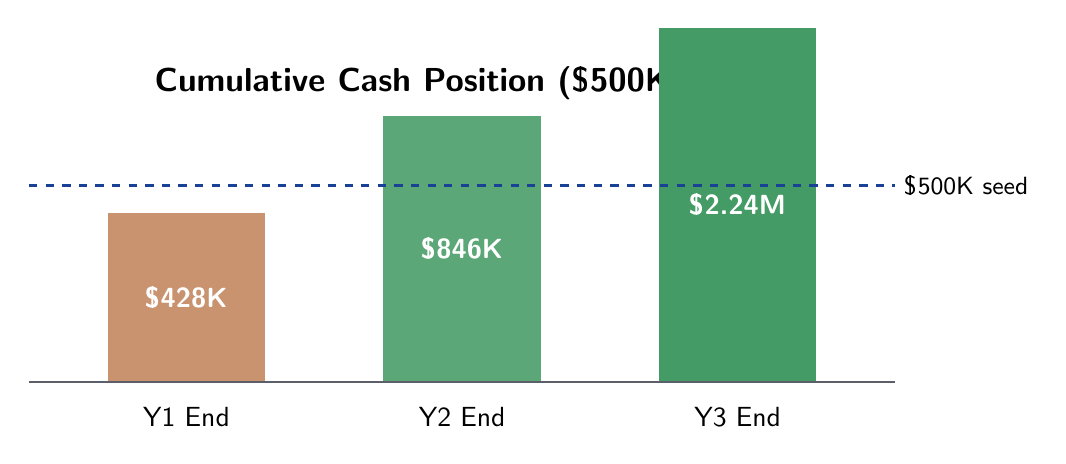
\begin{tikzpicture}
    % Title
    \node[align=center] at (0,3.8) {\textbf{\large Cumulative Cash Position (\$500K Seed)}};

    % Bars
    \fill[warningorange!60] (-4.5,0) rectangle (-2.5,2.14);
    \node at (-3.5,1.07) {\textcolor{white}{\textbf{\$428K}}};
    \node[below] at (-3.5,-0.2) {Y1 End};

    \fill[successgreen!70] (-1,0) rectangle (1,3.38);
    \node at (0,1.69) {\textcolor{white}{\textbf{\$846K}}};
    \node[below] at (0,-0.2) {Y2 End};

    \fill[successgreen!80] (2.5,0) rectangle (4.5,4.5);
    \node at (3.5,2.25) {\textcolor{white}{\textbf{\$2.24M}}};
    \node[below] at (3.5,-0.2) {Y3 End};

    % Baseline
    \draw[line width=1pt, freegray] (-5.5,0) -- (5.5,0);

    % Reference line for seed
    \draw[dashed, line width=1pt, miloprimary] (-5.5,2.5) -- (5.5,2.5);
    \node[right] at (5.5,2.5) {\small \$500K seed};
\end{tikzpicture}
\end{center}

% ============================================================================
% CHAPTER 5: PRODUCT & TECHNOLOGY
% ============================================================================
\chapter{Product \& Technology}

\section{Production-Ready Technology Stack}

\begin{center}
\infobox{miloprimary}{
    {\Large\textcolor{miloprimary}{\textbf{Complete, Production-Ready Codebase}}}\\[10pt]
    Unlike most seed-stage startups, MILO has a \textbf{fully functional} iOS app and backend API. The technology is built, tested, and ready for launch---we're not asking for money to build a prototype.\\[10pt]
    \begin{minipage}[t]{0.48\textwidth}
        \textbf{iOS Frontend:}
        \begin{itemize}[leftmargin=1.2em, itemsep=2pt]
            \item SwiftUI (iOS 16+)
            \item 14,600+ lines of Swift code
            \item MVVM architecture
            \item Firebase Auth (Google, Apple, Email)
            \item StoreKit 2 subscriptions
            \item Actor-based async services
        \end{itemize}
    \end{minipage}
    \hfill
    \begin{minipage}[t]{0.48\textwidth}
        \textbf{Backend API:}
        \begin{itemize}[leftmargin=1.2em, itemsep=2pt]
            \item FastAPI 0.109.0 (Python 3.11)
            \item PostgreSQL + SQLAlchemy 2.0
            \item Async/await throughout
            \item Railway hosting
            \item Dual API versions (v1/v2)
            \item Comprehensive rate limiting
        \end{itemize}
    \end{minipage}
}
\end{center}

\section{AI/ML Integration}

\begin{center}
\renewcommand{\arraystretch}{1.4}
\begin{tabular}{>{\raggedright\arraybackslash}p{3.5cm} >{\raggedright\arraybackslash}p{4cm} >{\centering\arraybackslash}p{2.5cm} >{\centering\arraybackslash}p{3cm}}
\toprule
\rowcolor{miloprimary!15}
\textbf{Service} & \textbf{Use Case} & \textbf{Cost} & \textbf{Accuracy} \\
\midrule
Veryfi OCR v8 & Receipt data extraction & \$0.08/receipt & 99\%+ \\
\rowcolor{lightbg}
Gemini 2.0 Flash & Item categorization & \$0.001/receipt & 95\%+ \\
Gemini 2.0 Flash & Milo chat assistant & \$0.002/message & -- \\
\rowcolor{lightbg}
Gemini 2.0 Flash & Budget AI insights & \$0.002/insight & -- \\
\bottomrule
\end{tabular}
\end{center}

\section{Core Product Features}

\textbf{1. Receipt Scanning}
\begin{itemize}[leftmargin=2em, itemsep=3pt]
    \item Veryfi OCR v8 integration with 99\%+ accuracy
    \item Supports JPEG, PNG, and PDF formats
    \item Duplicate detection to prevent double-counting
    \item Extracts: store name, date, total, and line items
\end{itemize}

\textbf{2. Health Scoring System (Proprietary IP)}

\begin{center}
\renewcommand{\arraystretch}{1.3}
\begin{tabular}{>{\centering\arraybackslash}p{1.5cm} >{\raggedright\arraybackslash}p{2.5cm} >{\centering\arraybackslash}p{2.5cm} >{\raggedright\arraybackslash}p{6cm}}
\toprule
\rowcolor{miloprimary!15}
\textbf{Score} & \textbf{Rating} & \textbf{Color} & \textbf{Examples} \\
\midrule
\cellcolor{successgreen!30}5 & Excellent & Green & Fresh vegetables, fruits, water, plain nuts \\
\cellcolor{successgreen!15}4 & Good & Light Green & Whole grains, lean proteins, eggs, plain dairy \\
\cellcolor{warningorange!15}3 & Moderate & Yellow & Bread, pasta, cheese, some ready meals \\
\cellcolor{warningorange!30}2 & Fair & Orange & Processed meats, sweetened drinks, some snacks \\
\cellcolor{dangerred!15}1 & Poor & Red-Orange & Chips, candy, cookies, sodas, sugary cereals \\
\cellcolor{dangerred!30}0 & Avoid & Red & Alcohol, energy drinks, heavily processed foods \\
\cellcolor{freegray!15}null & Non-Food & Gray & Household, personal care, pet supplies \\
\bottomrule
\end{tabular}
\end{center}

\textbf{3. 17-Category Classification}

\begin{center}
\renewcommand{\arraystretch}{1.2}
\small
\begin{tabular}{>{\raggedright\arraybackslash}p{3.5cm} >{\raggedright\arraybackslash}p{3.5cm} >{\raggedright\arraybackslash}p{3.5cm} >{\raggedright\arraybackslash}p{3.5cm}}
\toprule
Fresh Produce & Meat \& Fish & Dairy \& Eggs & Bakery \\
\midrule
Pantry & Frozen & Ready Meals & Snacks \& Sweets \\
\midrule
Drinks (Water) & Drinks (Soft/Soda) & Alcohol & Tobacco \\
\midrule
Household & Personal Care & Baby \& Kids & Pet Supplies \\
\midrule
\multicolumn{4}{c}{Other (uncategorized)} \\
\bottomrule
\end{tabular}
\end{center}

\textbf{4. AI Budget Intelligence (NEW)}

\begin{itemize}[leftmargin=2em, itemsep=3pt]
    \item \textbf{AI Budget Suggestions} -- Analyzes 3-12 months of spending history to recommend realistic budgets with category allocations
    \item \textbf{Daily AI Check-ins} -- Friendly status updates with actionable tips (``You're 65\% through your budget with 12 days left'')
    \item \textbf{Instant Receipt Analysis} -- Shows budget impact immediately (``This trip uses 9\% of your monthly budget'')
    \item \textbf{Monthly AI Reports} -- Letter grades (A+ to F), wins, challenges, and next month focus
    \item \textbf{Caching Strategy} -- Suggestions cached 24h, check-ins 1/day, reports cached permanently
\end{itemize}

\textbf{5. Milo Chat Assistant}

\begin{itemize}[leftmargin=2em, itemsep=3pt]
    \item Powered by Gemini 2.0 Flash
    \item Streaming responses via Server-Sent Events (SSE)
    \item Context-aware with full spending history
    \item Belgian grocery store knowledge
    \item 100 messages/month (Gold), 200/month (Platinum)
\end{itemize}

\section{System Architecture}

\begin{center}
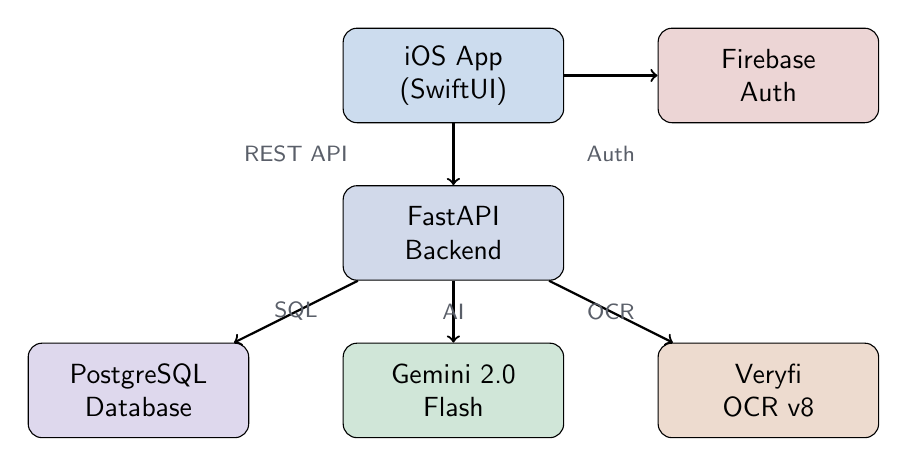
\begin{tikzpicture}[
    box/.style={draw, rounded corners=5pt, minimum width=2.8cm, minimum height=1.2cm, align=center},
    arrow/.style={->, thick}
]
    % iOS App
    \node[box, fill=appstoreblue!20] (ios) at (0,4) {iOS App\\(SwiftUI)};

    % Backend API
    \node[box, fill=miloprimary!20] (api) at (0,2) {FastAPI\\Backend};

    % Database
    \node[box, fill=datapurple!20] (db) at (-4,0) {PostgreSQL\\Database};

    % AI Services
    \node[box, fill=successgreen!20] (gemini) at (0,0) {Gemini 2.0\\Flash};

    % OCR
    \node[box, fill=warningorange!20] (veryfi) at (4,0) {Veryfi\\OCR v8};

    % Firebase
    \node[box, fill=dangerred!20] (firebase) at (4,4) {Firebase\\Auth};

    % Arrows
    \draw[arrow] (ios) -- (api);
    \draw[arrow] (ios) -- (firebase);
    \draw[arrow] (api) -- (db);
    \draw[arrow] (api) -- (gemini);
    \draw[arrow] (api) -- (veryfi);

    % Labels
    \node[freegray, font=\footnotesize] at (-2,3) {REST API};
    \node[freegray, font=\footnotesize] at (2,3) {Auth};
    \node[freegray, font=\footnotesize] at (-2,1) {SQL};
    \node[freegray, font=\footnotesize] at (0,1) {AI};
    \node[freegray, font=\footnotesize] at (2,1) {OCR};
\end{tikzpicture}
\end{center}

\section{API Endpoint Reference}

\begin{center}
\renewcommand{\arraystretch}{1.3}
\small
\begin{tabular}{>{\raggedright\arraybackslash}p{4.5cm} >{\raggedright\arraybackslash}p{5cm} >{\centering\arraybackslash}p{2.5cm}}
\toprule
\rowcolor{miloprimary!15}
\textbf{Endpoint} & \textbf{Description} & \textbf{Rate Limit} \\
\midrule
POST /receipts/upload & Upload receipt image & 25-50/month \\
\rowcolor{lightbg}
GET /receipts & List grouped receipts & -- \\
DELETE /receipts/\{id\} & Delete receipt & -- \\
\rowcolor{lightbg}
GET /transactions & List transactions & -- \\
PUT /transactions/\{id\} & Update transaction & -- \\
\rowcolor{lightbg}
POST /chat/stream & Streaming AI chat & 100-200/month \\
GET /budgets & Get user budget & -- \\
\rowcolor{lightbg}
POST /budgets & Create/update budget & -- \\
GET /budgets/ai-suggestion & AI budget recommendation & Cached 24h \\
\rowcolor{lightbg}
GET /budgets/ai-check-in & Daily AI check-in & 1/day \\
POST /budgets/ai-analyze-receipt & Instant receipt feedback & -- \\
\rowcolor{lightbg}
GET /budgets/ai-month-report & Monthly AI report & Cached \\
GET /analytics/summary & Spending summary & -- \\
\rowcolor{lightbg}
GET /analytics/categories & Category breakdown & -- \\
GET /analytics/trends & Spending trends & -- \\
\bottomrule
\end{tabular}
\end{center}

% ============================================================================
% CHAPTER 6: UNIT ECONOMICS
% ============================================================================
\chapter{Unit Economics \& Cost Structure}

\section{Variable Costs Per User}

\begin{center}
\renewcommand{\arraystretch}{1.5}
\begin{tabular}{>{\raggedright\arraybackslash}p{4cm} >{\centering\arraybackslash}p{2cm} >{\centering\arraybackslash}p{2cm} >{\centering\arraybackslash}p{3cm}}
\toprule
\rowcolor{miloprimary!15}
\textbf{Component} & \textbf{Gold} & \textbf{Platinum} & \textbf{Cost Basis} \\
\midrule
\textbf{Monthly Limits} & & & \\
\quad Receipts & 25 & 50 & -- \\
\rowcolor{lightbg}
\quad AI Chat Messages & 100 & 200 & -- \\
\midrule
\textbf{Variable Costs} & & & \\
\rowcolor{lightbg}
\quad Veryfi OCR (\$0.08/receipt) & \$2.00 & \$4.00 & Per receipt \\
\quad Gemini categorization & \$0.03 & \$0.05 & \$0.001/receipt \\
\rowcolor{lightbg}
\quad Gemini chat & \$0.20 & \$0.40 & \$0.002/message \\
\quad Firebase/storage & \$0.05 & \$0.10 & Per user/month \\
\midrule
\rowcolor{warningorange!10}
\textbf{Total Variable Cost/Month} & \textbf{\$2.28} & \textbf{\$4.55} & -- \\
\midrule
\textbf{Revenue/Month} & \$5.99 & \$12.99 & -- \\
\rowcolor{lightbg}
\textbf{Apple Fee (15\%)} & \$0.90 & \$1.95 & -- \\
\textbf{Net Revenue} & \$5.09 & \$11.04 & -- \\
\midrule
\rowcolor{successgreen!10}
\textbf{Contribution Margin} & \textbf{\$2.81} & \textbf{\$6.49} & -- \\
\rowcolor{successgreen!15}
\textbf{Contribution Margin \%} & \textbf{55\%} & \textbf{59\%} & -- \\
\bottomrule
\end{tabular}
\end{center}

\section{Customer Lifetime Value (LTV)}

\begin{center}
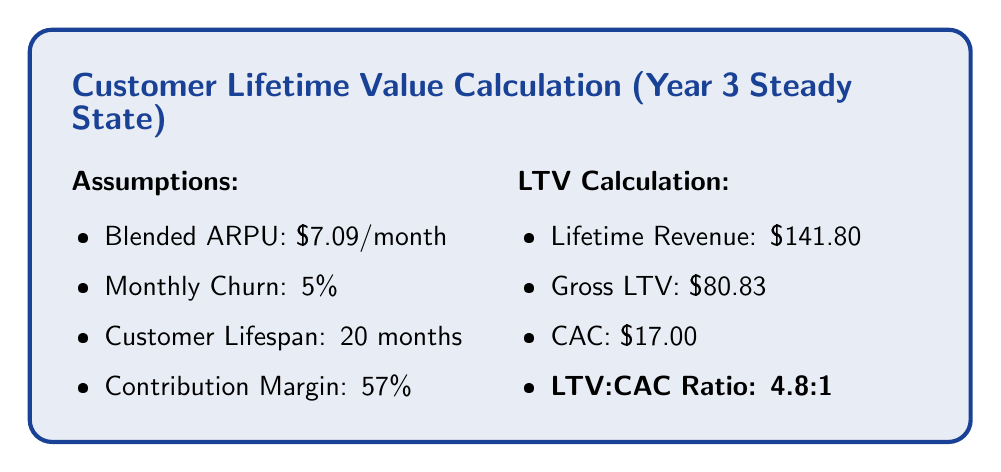
\begin{tikzpicture}
    \node[fill=miloprimary!10, draw=miloprimary, line width=1.5pt, rounded corners=8pt,
          inner sep=15pt, text width=\textwidth-35pt, align=left] {
        \textcolor{miloprimary}{\textbf{\large Customer Lifetime Value Calculation (Year 3 Steady State)}}\\[10pt]
        \begin{minipage}[t]{0.48\textwidth}
            \textbf{Assumptions:}
            \begin{itemize}[leftmargin=1.2em, itemsep=2pt]
                \item Blended ARPU: \$7.09/month
                \item Monthly Churn: 5\%
                \item Customer Lifespan: 20 months
                \item Contribution Margin: 57\%
            \end{itemize}
        \end{minipage}
        \hfill
        \begin{minipage}[t]{0.48\textwidth}
            \textbf{LTV Calculation:}
            \begin{itemize}[leftmargin=1.2em, itemsep=2pt]
                \item Lifetime Revenue: \$141.80
                \item Gross LTV: \$80.83
                \item CAC: \$17.00
                \item \textbf{LTV:CAC Ratio: 4.8:1}
            \end{itemize}
        \end{minipage}
    };
\end{tikzpicture}
\end{center}

\vspace{0.5cm}

\begin{center}
\renewcommand{\arraystretch}{1.4}
\begin{tabular}{>{\raggedright\arraybackslash}p{3cm} >{\centering\arraybackslash}p{2cm} >{\centering\arraybackslash}p{2.5cm} >{\centering\arraybackslash}p{2cm} >{\centering\arraybackslash}p{2cm} >{\centering\arraybackslash}p{2cm}}
\toprule
\rowcolor{miloprimary!15}
\textbf{Tier} & \textbf{Price} & \textbf{Lifetime Rev} & \textbf{Gross LTV} & \textbf{CAC} & \textbf{LTV:CAC} \\
\midrule
\rowcolor{goldcolor!8}
\textcolor{goldcolor}{\textbf{Gold}} & \$5.99/mo & \$101.83 & \$50.92 & \$17 & 3.0:1 \\
\rowcolor{platinumcolor!8}
\textcolor{platinumcolor}{\textbf{Platinum}} & \$12.99/mo & \$220.83 & \$121.48 & \$17 & 7.1:1 \\
\midrule
\rowcolor{successgreen!10}
\textbf{Blended Average} & \$7.09/mo & \$141.80 & \$61.51 & \$17 & \textbf{3.6:1} \\
\bottomrule
\end{tabular}
\end{center}

\vspace{0.3cm}

\begin{center}
\sourcebox{LTV:CAC benchmark of 3:1+ for healthy SaaS: SaaStr, ChartMogul industry standards; Churn assumptions based on RevenueCat State of Subscription Apps 2025}
\end{center}

\begin{center}
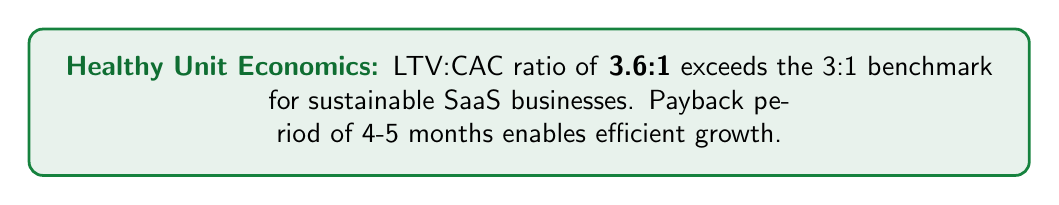
\begin{tikzpicture}
    \node[fill=successgreen!10, draw=successgreen, line width=1pt, rounded corners=5pt,
          inner sep=10pt, text width=12cm, align=center] {
        \textcolor{darkgreen}{\textbf{Healthy Unit Economics:}} LTV:CAC ratio of \textbf{3.6:1} exceeds the 3:1 benchmark\\for sustainable SaaS businesses. Payback period of 4-5 months enables efficient growth.
    };
\end{tikzpicture}
\end{center}

% ============================================================================
% CHAPTER 7: RISK ANALYSIS
% ============================================================================
\chapter{Risk Analysis \& Mitigation}

\section{Sensitivity Analysis}

\begin{center}
\renewcommand{\arraystretch}{1.4}
\begin{tabular}{>{\raggedright\arraybackslash}p{4cm} >{\centering\arraybackslash}p{2cm} >{\centering\arraybackslash}p{2cm} >{\centering\arraybackslash}p{2cm} >{\centering\arraybackslash}p{2cm}}
\toprule
\rowcolor{miloprimary!15}
\textbf{Variable} & \textbf{-20\%} & \textbf{Base Case} & \textbf{+20\%} & \textbf{Impact} \\
\midrule
\rowcolor{dangerred!10}
Trial Conversion Rate & \$950K & \$1.39M & \$1.83M & \cellcolor{dangerred!20}\textbf{HIGH} \\
\rowcolor{dangerred!10}
Data Consent Rate & \$1.14M & \$1.39M & \$1.64M & \cellcolor{dangerred!20}\textbf{HIGH} \\
\rowcolor{warningorange!10}
User Churn Rate & \$1.67M & \$1.39M & \$1.11M & \cellcolor{warningorange!20}MEDIUM \\
\rowcolor{warningorange!10}
Veryfi OCR Costs & \$1.41M & \$1.39M & \$1.37M & \cellcolor{successgreen!20}LOW \\
\rowcolor{successgreen!10}
Engineering Costs & \$1.45M & \$1.39M & \$1.33M & \cellcolor{successgreen!20}LOW \\
\bottomrule
\end{tabular}
\end{center}

\section{Scenario Analysis}

\begin{center}
\renewcommand{\arraystretch}{1.4}
\begin{tabular}{>{\raggedright\arraybackslash}p{3.5cm} >{\centering\arraybackslash}p{2cm} >{\centering\arraybackslash}p{2cm} >{\centering\arraybackslash}p{2cm} >{\centering\arraybackslash}p{2cm} >{\centering\arraybackslash}p{1.5cm}}
\toprule
\rowcolor{miloprimary!15}
\textbf{Scenario} & \textbf{Year 1} & \textbf{Year 2} & \textbf{Year 3} & \textbf{3-Yr Total} & \textbf{Prob.} \\
\midrule
\rowcolor{dangerred!10}
\textbf{Bear Case} & (\$150K) & \$150K & \$600K & \$600K & 20\% \\
\rowcolor{lightbg}
\textbf{Base Case} & (\$72K) & \$418K & \$1.39M & \$1.74M & 60\% \\
\rowcolor{successgreen!10}
\textbf{Bull Case} & \$50K & \$700K & \$2.2M & \$2.95M & 20\% \\
\midrule
\rowcolor{miloprimary!10}
\textbf{Expected Value} & (\$54K) & \$407K & \$1.37M & \textbf{\$1.72M} & -- \\
\bottomrule
\end{tabular}
\end{center}

\section{Key Risks \& Mitigations}

\begin{center}
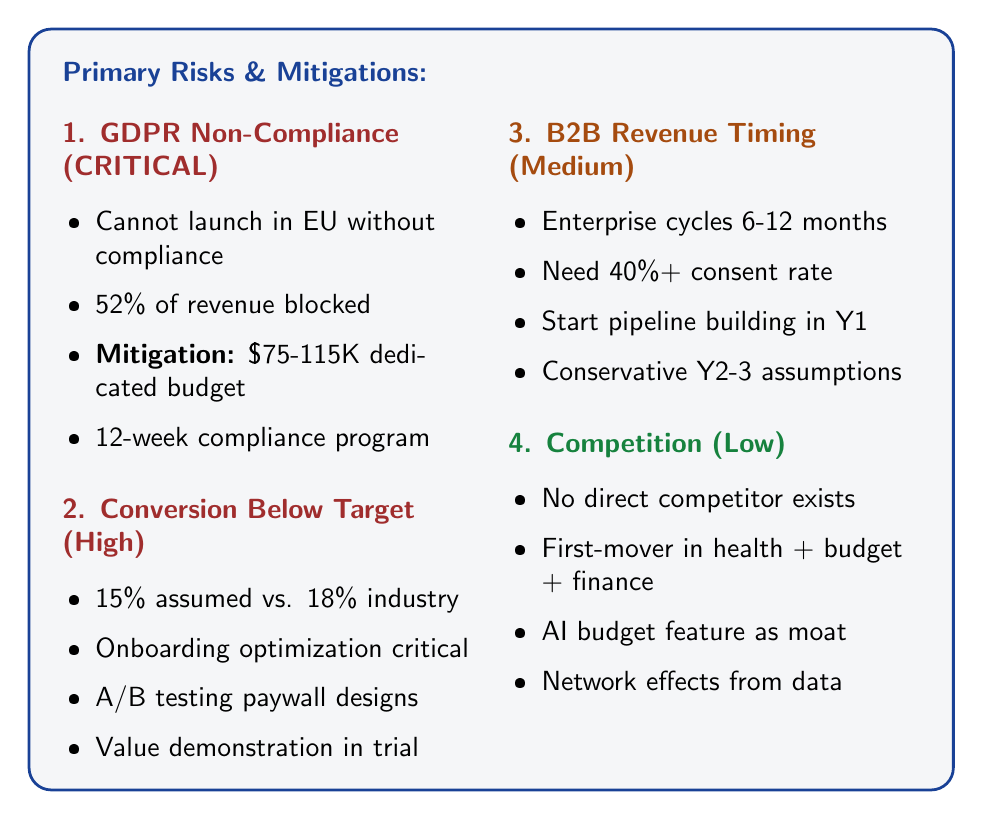
\begin{tikzpicture}
    \node[fill=lightbg, draw=miloprimary, line width=1pt, rounded corners=8pt,
          inner sep=12pt, text width=\textwidth-35pt, align=left] {
        \textcolor{miloprimary}{\textbf{Primary Risks \& Mitigations:}}\\[10pt]
        \begin{minipage}[t]{0.48\textwidth}
            \textcolor{dangerred}{\textbf{1. GDPR Non-Compliance (CRITICAL)}}
            \begin{itemize}[leftmargin=1.2em, itemsep=2pt]
                \item Cannot launch in EU without compliance
                \item 52\% of revenue blocked
                \item \textbf{Mitigation:} \$75-115K dedicated budget
                \item 12-week compliance program
            \end{itemize}
            \vspace{6pt}
            \textcolor{dangerred}{\textbf{2. Conversion Below Target (High)}}
            \begin{itemize}[leftmargin=1.2em, itemsep=2pt]
                \item 15\% assumed vs. 18\% industry
                \item Onboarding optimization critical
                \item A/B testing paywall designs
                \item Value demonstration in trial
            \end{itemize}
        \end{minipage}
        \hfill
        \begin{minipage}[t]{0.48\textwidth}
            \textcolor{warningorange}{\textbf{3. B2B Revenue Timing (Medium)}}
            \begin{itemize}[leftmargin=1.2em, itemsep=2pt]
                \item Enterprise cycles 6-12 months
                \item Need 40\%+ consent rate
                \item Start pipeline building in Y1
                \item Conservative Y2-3 assumptions
            \end{itemize}
            \vspace{6pt}
            \textcolor{successgreen}{\textbf{4. Competition (Low)}}
            \begin{itemize}[leftmargin=1.2em, itemsep=2pt]
                \item No direct competitor exists
                \item First-mover in health + budget + finance
                \item AI budget feature as moat
                \item Network effects from data
            \end{itemize}
        \end{minipage}
    };
\end{tikzpicture}
\end{center}

\section{Technical Risk Mitigations}

\begin{center}
\renewcommand{\arraystretch}{1.4}
\begin{tabular}{>{\raggedright\arraybackslash}p{4cm} >{\centering\arraybackslash}p{2cm} >{\raggedright\arraybackslash}p{7cm}}
\toprule
\rowcolor{miloprimary!15}
\textbf{Risk} & \textbf{Impact} & \textbf{Mitigation} \\
\midrule
Veryfi API cost increase & HIGH & Volume contracts, Google Document AI as backup \\
\rowcolor{lightbg}
Gemini API reliability & MEDIUM & Claude API fallback (already integrated in V1) \\
Firebase Auth issues & LOW & Token caching, Keychain storage, App Group sharing \\
\rowcolor{lightbg}
Database scaling & LOW & PostgreSQL indexing, connection pooling, Railway auto-scaling \\
\bottomrule
\end{tabular}
\end{center}

% ============================================================================
% CHAPTER 8: COMPLIANCE & LEGAL
% ============================================================================
\chapter{Compliance \& Legal}

\section{GDPR Compliance Status}

\begin{center}
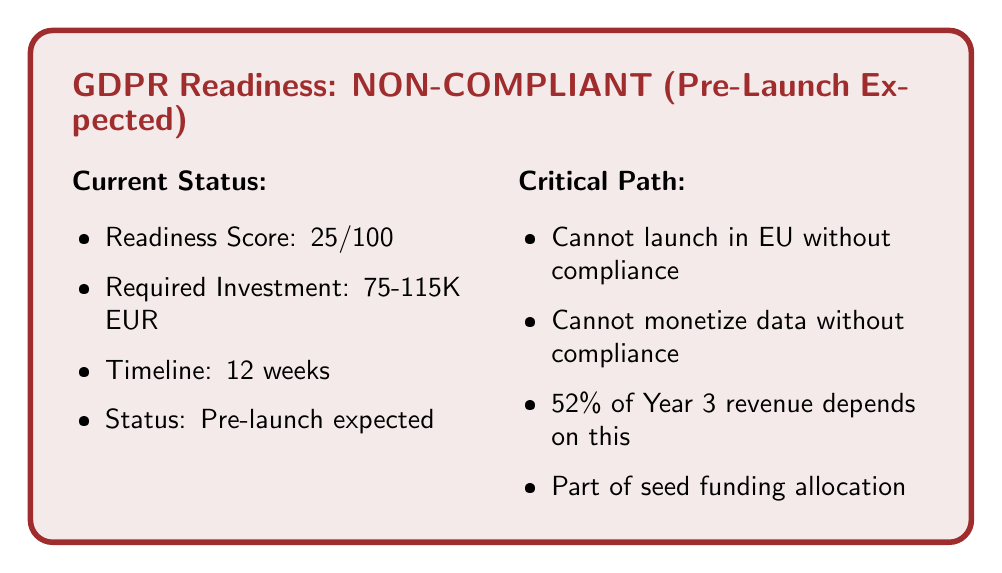
\begin{tikzpicture}
    \node[fill=dangerred!10, draw=dangerred, line width=2pt, rounded corners=8pt,
          inner sep=15pt, text width=\textwidth-35pt, align=left] {
        \textcolor{dangerred}{\textbf{\large GDPR Readiness: NON-COMPLIANT (Pre-Launch Expected)}}\\[10pt]
        \begin{minipage}[t]{0.48\textwidth}
            \textbf{Current Status:}
            \begin{itemize}[leftmargin=1.2em, itemsep=2pt]
                \item Readiness Score: 25/100
                \item Required Investment: 75-115K EUR
                \item Timeline: 12 weeks
                \item Status: Pre-launch expected
            \end{itemize}
        \end{minipage}
        \hfill
        \begin{minipage}[t]{0.48\textwidth}
            \textbf{Critical Path:}
            \begin{itemize}[leftmargin=1.2em, itemsep=2pt]
                \item Cannot launch in EU without compliance
                \item Cannot monetize data without compliance
                \item 52\% of Year 3 revenue depends on this
                \item Part of seed funding allocation
            \end{itemize}
        \end{minipage}
    };
\end{tikzpicture}
\end{center}

\section{Compliance Investment Required}

\begin{center}
\renewcommand{\arraystretch}{1.4}
\begin{tabular}{>{\raggedright\arraybackslash}p{5cm} >{\centering\arraybackslash}p{3cm} >{\centering\arraybackslash}p{3cm}}
\toprule
\rowcolor{miloprimary!15}
\textbf{Requirement} & \textbf{Investment} & \textbf{Priority} \\
\midrule
Privacy Policy \& Terms & 5-10K EUR & Critical \\
\rowcolor{lightbg}
Data Processing Agreements & 15-25K EUR & Critical \\
Consent Management System & 10-15K EUR & Critical \\
\rowcolor{lightbg}
Data Subject Rights Portal & 15-20K EUR & High \\
International Transfer Docs & 10-15K EUR & High \\
\rowcolor{lightbg}
DPIA for AI Processing & 10-15K EUR & High \\
Ongoing DPO Services & 10-15K EUR/year & Medium \\
\midrule
\rowcolor{warningorange!10}
\textbf{Total Initial Investment} & \textbf{75-115K EUR} & -- \\
\bottomrule
\end{tabular}
\end{center}

\section{Data Privacy Architecture}

\begin{itemize}[leftmargin=2em, itemsep=4pt]
    \item \textbf{Consent-First Model} -- Explicit opt-in required for data monetization
    \item \textbf{Tiered Consent} -- Users choose level of data sharing
    \item \textbf{Anonymization Pipeline} -- Personal identifiers removed before B2B use
    \item \textbf{Data Minimization} -- Only collect what's necessary for features
    \item \textbf{Right to Erasure} -- Full deletion capability implemented
    \item \textbf{Data Portability} -- Export feature for user data
\end{itemize}

% ============================================================================
% CHAPTER 9: INVESTMENT THESIS
% ============================================================================
\chapter{Investment Thesis}

\section{Investment Summary}

\begin{center}
\infobox{miloprimary}{
    {\Large\textcolor{miloprimary}{\textbf{Investment Opportunity (Conservative)}}}\\[12pt]
    \begin{minipage}[t]{0.48\textwidth}
        \textbf{Investment Details:}
        \begin{itemize}[leftmargin=1.2em, itemsep=2pt]
            \item Amount: \$400K - \$600K
            \item Round: Seed
            \item Runway: 18-24 months
            \item Break-even: Month 14
        \end{itemize}
    \end{minipage}
    \hfill
    \begin{minipage}[t]{0.48\textwidth}
        \textbf{Return Potential:}
        \begin{itemize}[leftmargin=1.2em, itemsep=2pt]
            \item Year 3 Revenue: \$2.4M
            \item Operating Margin: 58\%
            \item Valuation (6x): \$14.4M
            \item Return: 6-10x (conservative)
        \end{itemize}
    \end{minipage}
}
\end{center}

\section{Use of Funds (\$500K Mid-Point)}

\begin{center}
\renewcommand{\arraystretch}{1.4}
\begin{tabular}{>{\raggedright\arraybackslash}p{4cm} >{\centering\arraybackslash}p{1.5cm} >{\centering\arraybackslash}p{2.5cm} >{\raggedright\arraybackslash}p{5cm}}
\toprule
\rowcolor{miloprimary!15}
\textbf{Category} & \textbf{\%} & \textbf{Amount} & \textbf{Purpose} \\
\midrule
Product Development & 30\% & \$150K & Android, UK localization, B2B features \\
\rowcolor{lightbg}
Legal \& Compliance & 20\% & \$100K & GDPR, privacy, data agreements \\
User Acquisition & 20\% & \$100K & Marketing, influencers, paid acquisition \\
\rowcolor{lightbg}
B2B Sales & 15\% & \$75K & Sales team, partnerships \\
Operations & 15\% & \$75K & Finance, HR, contingency \\
\bottomrule
\end{tabular}
\end{center}

\section{Why Invest in MILO}

\begin{enumerate}[leftmargin=2em, itemsep=4pt]
    \item \textbf{Category Creator} -- First wellness-aware spending analytics platform
    \item \textbf{Production Ready} -- Complete iOS + FastAPI stack, not a prototype
    \item \textbf{AI-Native} -- Gemini 2.0 Flash at \$0.002/interaction
    \item \textbf{Sustainable Economics} -- 58\% operating margins, 3.6:1 LTV:CAC
    \item \textbf{Diversified Revenue} -- Three pillars reduce concentration risk
    \item \textbf{Capital Efficient} -- Profitable by Month 14, 18-24mo runway
    \item \textbf{Strong Moat} -- AI budget intelligence + health scoring + data network
\end{enumerate}

\section{Exit Valuation (Year 3)}

\begin{center}
\renewcommand{\arraystretch}{1.4}
\begin{tabular}{>{\raggedright\arraybackslash}p{3cm} >{\centering\arraybackslash}p{2cm} >{\centering\arraybackslash}p{3cm} >{\centering\arraybackslash}p{3cm}}
\toprule
\rowcolor{miloprimary!15}
\textbf{Scenario} & \textbf{Multiple} & \textbf{Valuation} & \textbf{Seed Return} \\
\midrule
\rowcolor{dangerred!10}
Conservative & 5x & \$12M & 3-4x \\
\rowcolor{lightbg}
\textbf{Base Case} & \textbf{6x} & \textbf{\$14.4M} & \textbf{6-8x} \\
Moderate & 8x & \$19.2M & 10-12x \\
\rowcolor{successgreen!10}
Optimistic & 10x & \$24M & 12-15x \\
\bottomrule
\end{tabular}
\end{center}

\section{Potential Acquirers}

\begin{center}
\renewcommand{\arraystretch}{1.4}
\begin{tabular}{>{\raggedright\arraybackslash}p{4cm} >{\raggedright\arraybackslash}p{8cm}}
\toprule
\rowcolor{miloprimary!15}
\textbf{Category} & \textbf{Companies} \\
\midrule
CPG \& Consumer (Most Likely) & Nestl\'{e}, P\&G, Unilever, PepsiCo, Kraft Heinz \\
\rowcolor{lightbg}
Data \& Analytics & NielsenIQ, Circana (IRI), Dun \& Bradstreet \\
Fintech \& Payments & Plaid, Yodlee, MX, Block (Square) \\
\rowcolor{lightbg}
Retail \& E-commerce & Instacart, Walmart Labs, Kroger Technology \\
\bottomrule
\end{tabular}
\end{center}

\section{Key Success Metrics}

\begin{center}
\renewcommand{\arraystretch}{1.5}
\begin{tabular}{>{\centering\arraybackslash}p{1cm} >{\raggedright\arraybackslash}p{5cm} >{\centering\arraybackslash}p{3cm} >{\raggedright\arraybackslash}p{5cm}}
\toprule
\rowcolor{miloprimary!15}
\textbf{\#} & \textbf{Metric} & \textbf{Target} & \textbf{Impact} \\
\midrule
1 & Trial-to-Paid Conversion & $\geq$ 15\% & Drives all B2C revenue \\
\rowcolor{lightbg}
2 & Monthly Churn & $\leq$ 5.5\% & Protects customer LTV \\
3 & Data Consent Rate & $\geq$ 40\% & Enables B2B revenue stream \\
\rowcolor{lightbg}
4 & Customer Acquisition Cost & $\leq$ \$20 & Maintains healthy unit economics \\
5 & GDPR Compliance & Complete by Q2 & Enables EU launch \\
\bottomrule
\end{tabular}
\end{center}

% ============================================================================
% CHAPTER 10: RESEARCH SOURCES
% ============================================================================
\chapter{Research Sources \& Methodology}

\section{Market Size \& Growth Data}

\begin{center}
\renewcommand{\arraystretch}{1.4}
\begin{tabular}{>{\raggedright\arraybackslash}p{4cm} >{\raggedright\arraybackslash}p{6cm} >{\raggedright\arraybackslash}p{4cm}}
\toprule
\rowcolor{miloprimary!15}
\textbf{Data Point} & \textbf{Source} & \textbf{Date} \\
\midrule
Receipt scanner market: \$2.5B (2025) & Growth Market Reports & 2024 \\
\rowcolor{lightbg}
Market CAGR: 11.1\% & Market Intelo & 2024 \\
Personal finance apps: \$7.2B & Statista & 2025 \\
\rowcolor{lightbg}
Consumer data analytics: \$12B & Fortune Business Insights & 2025 \\
Data analytics CAGR: 22\% & Fortune Business Insights & 2025 \\
\rowcolor{lightbg}
Health/wellness market: \$7.32T & Global Wellness Institute & 2025 \\
\bottomrule
\end{tabular}
\end{center}

\section{Consumer Behavior Data}

\begin{center}
\renewcommand{\arraystretch}{1.4}
\begin{tabular}{>{\raggedright\arraybackslash}p{5cm} >{\raggedright\arraybackslash}p{5cm} >{\raggedright\arraybackslash}p{3.5cm}}
\toprule
\rowcolor{miloprimary!15}
\textbf{Data Point} & \textbf{Source} & \textbf{Date} \\
\midrule
85\% check nutrition labels & IFIC Food \& Health Survey & 2024 \\
\rowcolor{lightbg}
71\% trying to improve diet & IFIC Food \& Health Survey & 2024 \\
67\% pay more for health claims & NielsenIQ Wellness Trends & 2024 \\
\rowcolor{lightbg}
16\%+ households with GLP-1 user & KFF Health Tracking Poll & May 2024 \\
6\% of adults on GLP-1 drugs & KFF Health Tracking Poll & May 2024 \\
\rowcolor{lightbg}
3.6M Mint active users & Bloomberg & 2021 \\
Mint shutdown: March 2024 & CNBC Select & March 2024 \\
\rowcolor{lightbg}
41\% subscription fatigue & Various industry reports & 2025 \\
\bottomrule
\end{tabular}
\end{center}

\section{SaaS \& Mobile App Benchmarks}

\begin{center}
\renewcommand{\arraystretch}{1.4}
\begin{tabular}{>{\raggedright\arraybackslash}p{5cm} >{\raggedright\arraybackslash}p{5cm} >{\raggedright\arraybackslash}p{3.5cm}}
\toprule
\rowcolor{miloprimary!15}
\textbf{Benchmark} & \textbf{Source} & \textbf{Date} \\
\midrule
18.2\% opt-in trial conversion & First Page Sage & 2024 \\
\rowcolor{lightbg}
9\% mobile subscription churn & RevenueCat State of Apps & 2025 \\
3:1 LTV:CAC healthy ratio & SaaStr, ChartMogul & Industry standard \\
\rowcolor{lightbg}
20\% MoM ideal growth rate & OneSignal App Benchmarks & 2024 \\
\$25-75 panelist value/year & NielsenIQ, Circana & 2024 \\
\bottomrule
\end{tabular}
\end{center}

\section{Competitor Information}

All competitor pricing and feature information sourced directly from company websites as of January 2026:
\begin{itemize}[leftmargin=2em, itemsep=2pt]
    \item Fetch Rewards: \url{https://fetch.com/}
    \item Ibotta: \url{https://ibotta.com/}
    \item Copilot Money: \url{https://copilot.money/}
    \item Monarch Money: \url{https://www.monarchmoney.com/}
    \item Yuka: \url{https://yuka.io/}
\end{itemize}

\vspace{1cm}

% ============================================================================
% CONCLUSION
% ============================================================================
\begin{center}
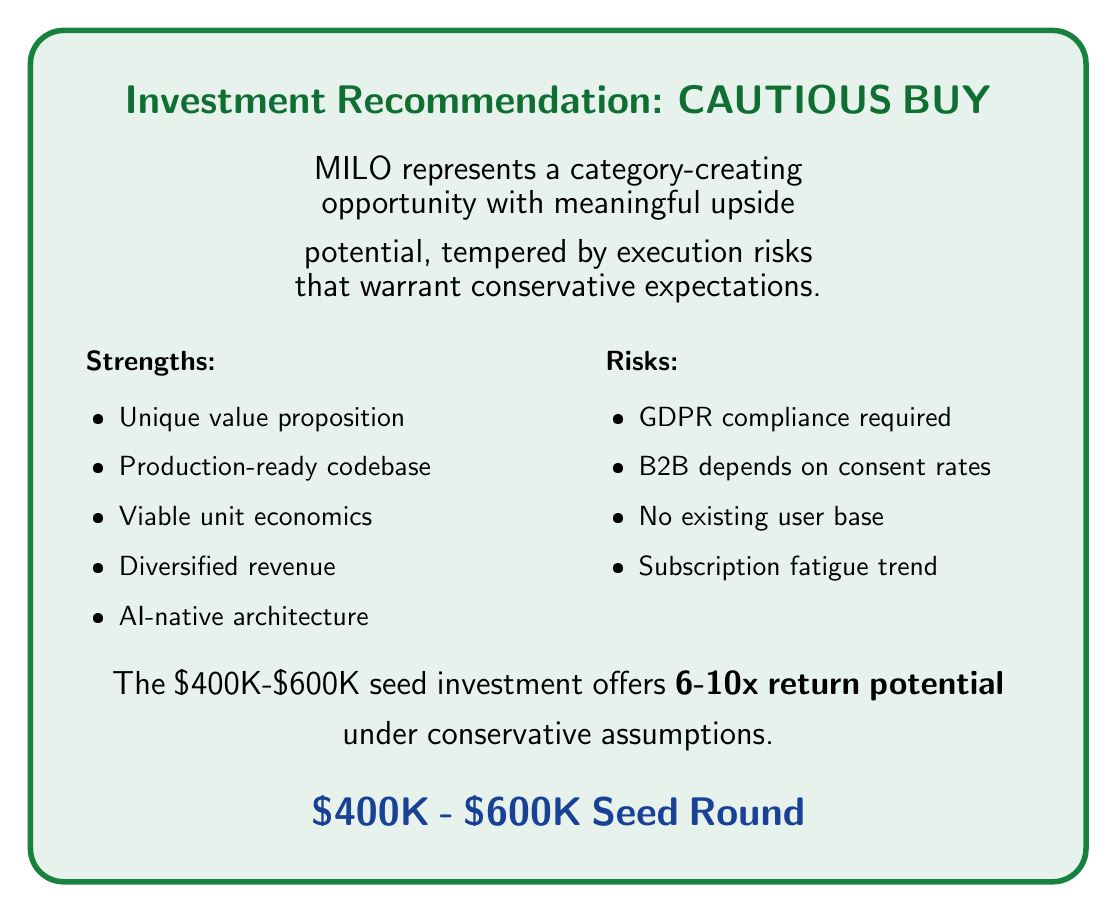
\begin{tikzpicture}
    \node[fill=successgreen!10, draw=successgreen, line width=2pt, rounded corners=12pt,
          inner sep=20pt, text width=12cm, align=center] {
        {\Large\textcolor{darkgreen}{\textbf{Investment Recommendation: CAUTIOUS BUY}}}\\[12pt]
        {\large MILO represents a category-creating opportunity with meaningful upside}\\[6pt]
        {\large potential, tempered by execution risks that warrant conservative expectations.}\\[15pt]
        \begin{minipage}[t]{0.45\textwidth}
            \textbf{Strengths:}
            \begin{itemize}[leftmargin=1.2em, itemsep=2pt]
                \item Unique value proposition
                \item Production-ready codebase
                \item Viable unit economics
                \item Diversified revenue
                \item AI-native architecture
            \end{itemize}
        \end{minipage}
        \hfill
        \begin{minipage}[t]{0.45\textwidth}
            \textbf{Risks:}
            \begin{itemize}[leftmargin=1.2em, itemsep=2pt]
                \item GDPR compliance required
                \item B2B depends on consent rates
                \item No existing user base
                \item Subscription fatigue trend
            \end{itemize}
        \end{minipage}\\[15pt]
        {\large The \$400K-\$600K seed investment offers \textbf{6-10x return potential}}\\[6pt]
        {\large under conservative assumptions.}\\[15pt]
        {\Large\textcolor{miloprimary}{\textbf{\$400K - \$600K Seed Round}}}
    };
\end{tikzpicture}
\end{center}

\vspace{1.5cm}

% Footer
\begin{center}
    \textcolor{freegray}{\rule{12cm}{0.5pt}}\\[0.4cm]
    \textcolor{freegray}{\small DeepmAInd B.V. | Confidential | Version 4.0 | January 2026}\\[0.2cm]
    \textcolor{freegray}{\scriptsize Conservative projections with research-backed growth assumptions}\\
    \textcolor{freegray}{\scriptsize Production-ready iOS + FastAPI with AI Budget Intelligence}
\end{center}

\end{document}
